% This is latex template version 0.1
\documentclass[twosided,times,11pt]{article}

\usepackage[draft]{djb}
\usepackage{shortcuts}
\usepackage{fancyhdr}

%%%%%%%%%%%%%%%%%%%%%%%%%%%%%%%%%%%%%%%%
%%% Scribes: you must fill these in %%%%
%%%%%%%%%%%%%%%%%%%%%%%%%%%%%%%%%%%%%%%%
\newcommand{\lecdate}{November 23, 2011}
\newcommand{\lectitle}{Differential GPS Attack Surface Analysis}
%%%%%%%%%%%%%%%%%%%%%%%%%%%%%%%%%%%%%%%%


\pagestyle{fancyplain}

\setlength{\headheight}{14pt}
\lhead[\fancyplain{}{\bfseries \thepage}]%
      {\fancyplain{}{\bfseries\lectitle}}
\chead[]{}
\rhead[\fancyplain{}{\bfseries\lectitle}]%
      {\fancyplain{}{\bfseries \thepage}}
\lfoot[{\small\scshape Project Writeup}]{{\small\scshape Project Writeup}}
\cfoot[]{}
\rfoot[{\small\scshape\lecdate}]{{\small\scshape\lecdate}}

\hypersetup{%
pdfauthor = {Brady Tello},
pdftitle = {\lectitle},
bookmarksopen= {true}
}

\begin{document}
\maketitle

\section{Introduction}

Modern civilian GPS receivers are capable of calculating their position on the Earth with accuracies on the order of meters.  This level of accuracy is not sufficient for many applications and thus a technique called differential GPS has been developed which provides sub-meter accuracy or better if configured properly.

Due to the nature of differential GPS systems, as discussed in Section 2, they often transmit positioning data over land based communication networks such as the Internet which makes them vulnerable to traditional network based attacks.  In this paper, we provide a list of attack vectors against a differential GPS system as well as a list of objectives that an attacker might have when targeting a differential GPS system.  We also discuss a concrete attack against a reference implementation of a differential GPS engine called rtknavi.  In our attack we were able to successfully control a GPS receivers reported position with some degree of accuracy by corrupting only differential GPS corrections.

In Section 2, we discuss differential GPS more thoroughly.  In section 3, we cover the standards which define the structure and transportation mechanisms for the data required in a differential GPS network.  Section 4 lists real applications of differential GPS systems.  Section 5 presents attack vectors against  a differential GPS network followed by a listing of speculative attack objectives in Section 6.  Our attack implementation is covered in Section 7 and the final part of our security analysis is in Section 8 where we discuss the Scope of Impact of our findings.

\section{Differential GPS}


Differential GPS or DGPS is a method for increasing the accuracy of ordinary
GPS.  Several factors contribute to error in GPS with a single receiver.  These
include ionospheric refraction of the GPS signal, noise, clock errors, and other
sources.  The idea behind DGPS is that a second receiver called a reference
station is placed in a known location and can measure the error between
the expected signal and the signal actually received.  The reference station
then transmits this difference to the roving receiver, which applies the
information to its position calculation.  The result is a more accurate
position calculation for the rover.  Applying DGPS to ordinary GPS can cause
the accuracy to improve from about 15 meters of error to about 2-3 centimeters
of error in the best case \cite{RTKWhitePaper} \cite{NTRIP1}.

DGPS is a term that applies to all types of GPS that have two or more receivers
for more accurate readings, but can be broken down into two categories, DGPS and
Kinematic GPS.  DGPS is the term usually applied to the types of Differential GPS 
that obtain meter level accuracy of readings.  Kinematic GPS is a different kind
of DGPS that can obtain accuracy within a few centimeters \cite{Heave}.  
Kinematic GPS requires five satellites to work properly and takes a minute to
initialize.  This is compared to the three or four satellites required to run
DGPS and no initialization time \cite{RTKWhitePaper}.  Though some of the
attacks described in this paper exploit Kinematic GPS, the term Differential
GPS or DGPS will be used to refer to the general idea of using more than one
receiver to calculate more accurate position.

\section{RTCM and Ntrip}

The Radio Technical Commission for Maritime Services (RTCM) is a non-profit organization comprised of both government and non-government bodies that publishes standards related to several topics including differential GPS.   RTCM�s Special Committee 104 publishes two standards which we focused on in our research.  

First we will discuss the RTCM 10403.1 standard (Differential GNSS Services Version 3).  The 10403.1 standard defines a set of messages which contain the data required by Differential GPS capable receivers\cite{RTCM3}.  The data defined by this standard is commonly referred to as just ``RTCM'', ``RTCM-104'', or ``RTCMv3''.  From this point on, we will refer to the data standard as RTCM unless it would be ambiguous in which case we will be careful to clarify the intended meaning.
\newline

\begin{figure}[h!]
	\centering
		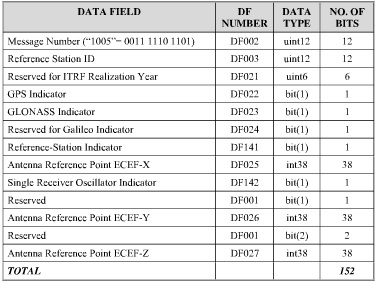
\includegraphics[scale=0.60]{RTCM1005.jpg}
	\caption{An Example of an RTCM Message}
\end{figure}

The second standard of interest is known as Ntrip (Networked Transport of RTCM over Internet Protocol) which is also published by the RTCM Special Committee 104.  Ntrip is an application layer networking protocol designed to stream RTCM correction data over the Internet.  A feature of Ntrip that seems to be popular is that it can transmit corrections over cellular data networks such as GPRS and EDGE, thus allowing corrections to be downloaded in very remote locations.  After conducting a survey of commercial GPS devices and conducting brief interviews with sources close to the development of Ntrip we have come to the conclusion that most commercial GPS reference stations are equipped with the capability to transmit RTCM correction data over Ntrip.  Furthermore, it has a wide variety of use cases which will be discussed in Section 4. The technical details of the protocol are contained in the following paragraphs.

The primary objective of the Ntrip protocol is to transmit correction data from reference stations to receivers over the Internet.  Its architecture is similar to that of a streaming Internet radio service.  When a GPS receiver wants to ``listen'' to a correction stream from a reference station, it requests the stream from a broadcast source which delivers the stream to the receiver in real time.  In Ntrip terminology a reference station is known as an Ntrip Source, a receiver is known as an Ntrip Client, and a broadcaster is known as an Ntrip Caster.  An additional component known as an Ntrip Server acts as a middle man between sources and casters.  The server aggregates data streams coming from sources and delivers them to casters which in turn aggregate several servers.
\newline

The standard is relatively abstract in its definitions of these components so it is helpful to understand how they might be implemented in a real Ntrip network.  An Ntrip source is simply a pseudonym for a GPS reference station such as the Trimble NetRS on which we conducted our experiments.  The device generates raw RTCM data which is uploaded to a server using one of several communications interfaces such as serial, TCP/IP, or various others (the Ntrip standard actually doesn�t define a communication interface between sources and servers).  An Ntrip Server and an Ntrip Caster are generally implemented as traditional software packages installed on one or more desktop/laptop computer(s).  Although they are defined as two logically separate entities, the server and caster can be implemented as part of the same program and still conform to the specification \cite{NTRIP2}.  A client is a piece of software at the end users receiver which is trying to correct its position.  A client downloads a list of reachable devices from the caster.  The list of devices is called a source table and contains entries for other casters, networks, and correction streams.  The Ntrip client downloads corrections and hands them off to the GPS software which then applies them to an uncorrected position in order to get a corrected, high precision, position. During our research we have found Ntrip client programs implemented on cell phones and devices known as data controllers, however, it would be perfectly reasonable to implement it directly on the receiver itself.


\begin{figure}[h!]
	\centering
		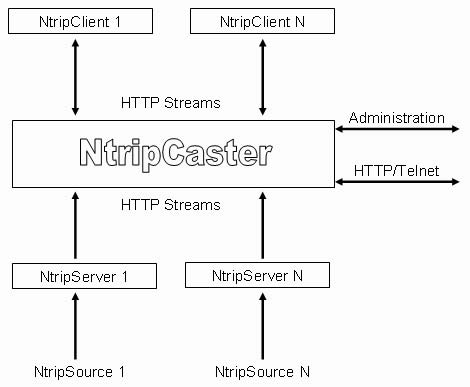
\includegraphics[scale=0.60]{ntripdiagram.jpg}
	\caption{Ntrip Protocol Architecture}
\end{figure}


The reason we have decided to focus our efforts on Ntrip and RTCM is because of their non-proprietary nature.  The two are not the only protocols available for encoding and disseminating differential correction data but they are certainly widely implemented and open to the general public (for a small fee).  Knowing that all differential GPS packages adhere to the same physical principles, we assume that they would be vulnerable in similar ways but this question is left for future work.

\section{Sample Applications}

This section will enumerate a subset of the possible applications of differential GPS.  The applications listed here are those for which we were able to determine that Ntrip is being used in some way.  One should refer to the National DGPS Assessment Report from the US Department of Transportation\cite{NDGPS1} for a more comprehensive list of the application domains of GPS in general.

\subsection{Machine Control}

Machine control is a sector of the GPS industry which aims to make construction projects more efficient and accurate.  In machine control, GPS receivers are hooked up to construction equipment such as bulldozers, scrapers, excavators, etc.  The GPS receivers assist equipment operators in things like maintaining consistent grades throughout a project.  For example, if a grader were too far off its mark, the GPS system could either warn the operator or make automatic corrections without operator assistance.  This saves time and money for a construction firm and would most likely increase the overall quality of their work.  By using differential GPS techniques,  the equipment can be made even more accurate \cite{TRIMBLE_MACH_CTRL}.

\subsection{Navigation}

Real time maritime and aerial navigation are two applications which are especially interesting.  Aerial navigation uses a differential GPS system called the Wide Area Augmentation system.  During our research of the NetRS device, we noticed that it can be configured to function as a WAAS reference station.  Since we have shown that the NetRS is vulnerable to compromise, this probably isn't a good thing.  The NDGPS assessment report contains an excellent list of real world applications of Differential GPS in the navigation domain \cite{NDGPS1}.

Automating your steering wheel is another interesting area in which high precision GPS could be used.  In \cite{Uradzinski:2010}, the use of Ntrip based RTK solutions was investigated for its use in automated collision avoidance for land based automobiles.  While this was only a research study, it shows that there are people who are interested in applying this technology to automated land based vehicle navigation.  Another example of such a system is the Cooperative Intersection Collision Avoidance System (CICAS) run by the US Dept. of Transportation and described in \cite{NDGPS1}

\subsection{Surveying}

Surveyors, by the nature of their profession, require the use of very precise position information and thus benefit greatly from the use of differential GPS technologies.  Surveyors often perform the task of staking out important geographical reference points.  To get an idea of the importance of the accuracy of reference points, imagine trying to build a house based on a reference point that was off by a foot.  If you didn't catch the mistake, your entire house would be shifted a foot from where you wanted it!  While, admittedly, this is a contrived example, it is simply meant to illustrate the types of errors that can occur if a surveyor is wrong.  The work of surveyors is broad in scope but it is fair enough to say that they are responsible for laying the basis for geographic measurements within a given context.  If they are wrong, everyone else will be wrong as well.

\subsection{Infrastructure Monitoring}

Monitoring of critical infrastructure such as bridges, tunnels, and dams is an important part of the professional surveying community.  Infrastructure monitoring involves installing high precision sensors in strategic locations on structures of interest.  The sensors generate position data which is compared against a set of movement thresholds.  If the thresholds are broken (the structure has shifted an unacceptable amount) a notification is delivered so that appropriate action can be taken\cite{TRIMBLE_INF_MON}.

\subsection{Early Warning Systems}

The University of California San Diego maintains a real time GPS network dedicated to researching ``early warning systems for natural disasters'' \cite{UCSD_RTN}.  The network is known as the California Real Time Network.  A brief survey of some of the documents found on the network's website indicate that the primary concern is earthquakes.

\section{Attack Vectors}

In this section, we will outline potential attack vectors against Ntrip networks.  These are mechanisms by which an attacker can influence the data received by an Ntrip client.  A list of objectives of these attacks is provided in Section 6.

\subsection{Security Statistics}

To assist us in our attack vector assessment, we have collected a small body of statistics regarding the security of Ntrip sources.  We wrote a script which scanned the list of casters provided at rtcm-ntrip.org to determine what kind of security is in place in the wild for Ntrip sources.  

Our script considered the Ntrip network as a directed cyclic graph with a ``root'' vertex at rtcm-ntrip.org which provides links to over 140 Ntrip casters\cite{NTRIP_BC_INFO} (22 of which we were unable to connect to).  The source table obtained from a vertex describes the edges leading to neighboring vertices.  Caster, and network entries in a  vertex's source table are considered branch nodes and source entries are considered leaves.  

The script we wrote performed a traversal to depth 1 in the graph, gathering statistics about each Ntrip source encountered including: device type, whether a fee is charged for accessing the source, and whether the device uses digest or basic authentication.  We chose to only go to depth 1 in the interest of time.  This gave us statistics on over 5000 source devices.  What we found is that only one of the streams required digest authentication, 867 of them assessed a fee, and that the Trimble NetRS was the most prevalent device found in the wild (22 percent of the devices we found were NetRS stations).

It should be noted that although this is a fair amount of data, it is likely only a small sampling of the total population of Ntrip sources.  Our script identified 291 caster links which it simply ignored.  Since we only scanned 119 casters, one can imagine how much data is still available.   

\subsection{Man in the middle}

The most serious attack vector we have identified is a man in the middle attack between casters and clients.  If a skilled adversary could convince a client to connect to his malicious caster using any number of network based man in the middle attack tools such as the freely available Cain and Abel or the GRPS, EDGE, UMTS, HSPA targeted attack described in  \cite{BLACKHAT:2011}  he could easily spoof the Ntrip protocol and trick the client into using corrupted correction data.  This attack is possible due to the lack of mutual authentication between clients and casters in the Ntrip protocol.

We consider this the most dangerous of our attacks because it is equivalent to compromising the RTCM streams served by that caster.  This way, an attacker wouldn't have to worry about the receiver device ``averaging out'' a misbehaving stream (so far we have found no evidence of software that does this) as long as they spoofed all the streams to  misbehave identically.

\subsection{Authentication Spoofing}  

Authentication is used in Ntrip networks to access RTCM streams or administer casters/servers \cite{NTRIP1} \cite{NTRIP2}.  If an attacker can determine a valid set of credentials they could either access restricted services (described in the false billing section) or configure a caster/server in a malicious manner.

The Ntrip standards do not specify exactly how a caster/server must be implemented but they do state that administrators are responsible for registering devices with casters/servers.  If an attacker were to gain access to the administration interface he could register malicious servers with a legitimate caster or malicious sources with legitimate servers (which would propagate to the caster and client).

Casters have the option of specifying basic or digest authentication methods for accessing sources.  An initial thought was that we would have to find a way to crack digest authentication in order to access the sources.  After analyzing the results of our scan however, it is clear that this isn't really necessary in the vast majority of cases (assuming that our sample data is representative of the entire population).  Only a single stream out of nearly 5000 was protected by digest authentication.  A wise attacker would obviously reach for the low hanging fruit and simply monitor the network to obtain the base64 encoded credentials which can be trivially decoded using any number of web/client based tools.  We ran a Base64 decoder on the encoded credentials transmitted by a reference implementation of an Ntrip client and verified that the plaintext credentials are trivially retrieved.

Regarding the caster/server passwords we can't say how difficult it would be to obtain a set of credentials in every case.  The first Ntrip standard specifies that caster administration is performed using telnet which would be an easy target but the second version does not specify the exact administration method.  It is thus our recommendation that implementors choose a sufficiently secure authentication method in order to prevent against this type of attack.

\section{Attack Objectives}

In this section, we provide a list of potential objectives of an attack against a differential GPS system.  We believe that these would be realistic objectives for an attacker based on current real-life usage of GPS systems but are entirely speculative at this point.  We have no evidence showing that differential GPS systems have been exploited for these means.  Future work would further investigate the objectives of real attacks against differential GPS systems.

 \subsection{Economic Damage}
 
 Almost all of the attack objectives outlined in this section will cause some level of economic damage.  An attacker could destroy automatically piloted vehicles, cause faulty surveys resulting in wasted effort or damage to structural integrity, make false charges to an Ntrip subscribers account, etc.
 
Lax security in differential GPS means that the high precision guarantees might not be guarantees at all.  If enough people were to catch on to this fact, the entire industry could suffer as a result.

\subsection{Navigational Control Hijacking / Confusion}

In our attack against a reference RTK implementation described in Section 7, we have found that it is possible to control a receiver's position calculations with some degree of accuracy.  This is possible by spoofing the reported X and Y coordinates of a reference station in message 1005 of the RTCM3 stream.  If a concrete receiver implementation exhibited similar behavior, it would be possible to control automated navigation systems that use Ntrip.  For example, if a receiver were reporting positions that were 1 foot to the West of its actual location, any software using this data to correct its position would adjust its course 1 foot to the East.  This attack could be used to confuse or even control automated navigation systems.

\subsection{False Billing} 

Depending on the billing model used, an attacker could log excessive accesses to a legitimate user's account.  The billing models we encountered were all flat rate charges (per month) but one could imagine other pay-per-use systems.  For example, if a service provider charged a dollar for every MB of correction data downloaded, an attacker could cause financial damage to a subscriber.

\subsection{Alarm Control}

The use of differential GPS in infrastructure and environmental monitoring projects provides attackers with the ability to interfere with sensor alarms\cite{UCSD_RTN}.  If an adversary were to transmit correction data to a stationary sensor to make it believe that it were moving, this could generate a false alarm if the movement tolerance were to be surpassed.  The damages from such an attack would vary with the level of response to a sensor alarm.  The other possibility is alarm suppression.  In an attack targeted on alarm suppression, the attacker would displace a stationary sensor some distance $\Delta$ over a time period $ t $ while simultaneously feeding the receiver corrupted correction data to make it believe that its total displacement during $ t $ was equal to 0.  This attack would hide an attacker whose goal is to move sensors without being noticed.  This is similar to Stuxnet's technique of silencing critical sensors\cite{STUXNET}. 

\subsection{Location Privacy Violations}

Section 2.1.3 of the Ntrip version 2 standard describes functionality in which a client transmits its location information to a caster so that the caster can provide location aware services.  An attacker who can monitor the network or who has control of a caster can observe the position of a client which may not be acceptable in certain circumstances.

\section{An Attack on a Real Time Kinematics Engine}

\subsection{Attack Testbed}

A Real Time Kinematics Engine is a program that receives correction data
and applies that data to calculate its known position.  In this section we
present an attack against an RTK Engine as an example of a concrete example
of a vulnerability in DGPS.  Before we go into details of the attack on a
RTK Engine, we will first describe the testing environment we used.
\newline

In order to show how our attack works, we needed to set up an environment
eqivalent to that of a fully functioning Ntrip network.  We configured a
Linux virtual machine running an FTP server and a reference implementation
of a caster and server, downloaded from BKG's official Ntrip
site\cite{NTRIP_BC_INFO}. The Windows 7 host machine was running a program
called RTKNAVI as the Ntrip client.  RTKNAVI uses the RTKLIB opensource
library as an RTK engine.  We connect to the NetRS mountpoint over a TCP/IP
connection through the Linux virtual machine.

\subsection{The Attack In Action}

\begin{figure}[h!]
	\centering
	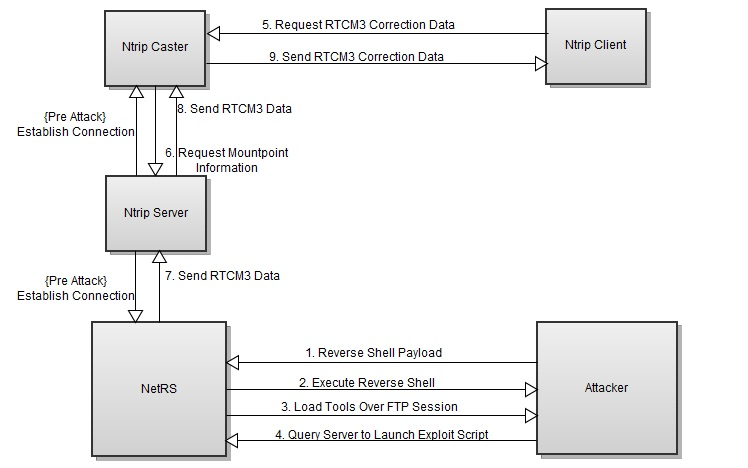
\includegraphics[scale=0.50]{attack-diagram.png}
	\caption{Attack Diagram}
\end{figure}

The attack began with two pre-attack conditions.  We launched our attack
while an Ntrip Caster was connected and exchanging data with an Ntrip
Server.  Simultaneously, our attack happened while the same Ntrip Server
was receiving streaming data from a NetRS mountpoint.


The first stage of the attack was to exploit the NetRS mountpoint.  The
NetRS device used an Apache module to run perl scripts through a web
interface.  Using a custom perl script as a payload to the NetRS device,
the attack machine successfully obtained a reverse shell on the mountpoint.
 The next goal was to construct and load tools to the NetRS mountpoint.
 The tools would launch a server on the NetRS to stream arbitrary RTCM3
correction data to a connecting Ntrip Server.  While on the NetRS device, a
few observations were made and diagnosed on how to progress.

The NetRS was running on a PowerPC architecture with very few pre-installed
programs, FTP being one.  To avoid cross-compilation issues and bypass the
lack of a Perl, Python, Ruby, Java, etc. interpreter, we decided to
leverage the use of the Apache Perl Module that we used to get the remote
shell.  After designing a Perl script to accomplish the next stage of our
attack, we opened an FTP session from the NetRS to the attacking machine to
load this tool.  The last stage of our attack was to execute the script via
the Apache Perl Module by accessing it through the NetRS web interface.

After the NetRS was configured to send the custom-made RTCM3 correction
data, the Ntrip Server reconnected to the NetRS and began to receive the
RTCM3 data streamed by the mountpoint.  The data propagated to the Ntrip
Caster where it waited for a connecting Ntrip Client to request this data.

\begin{figure}[h!]
	\centering
		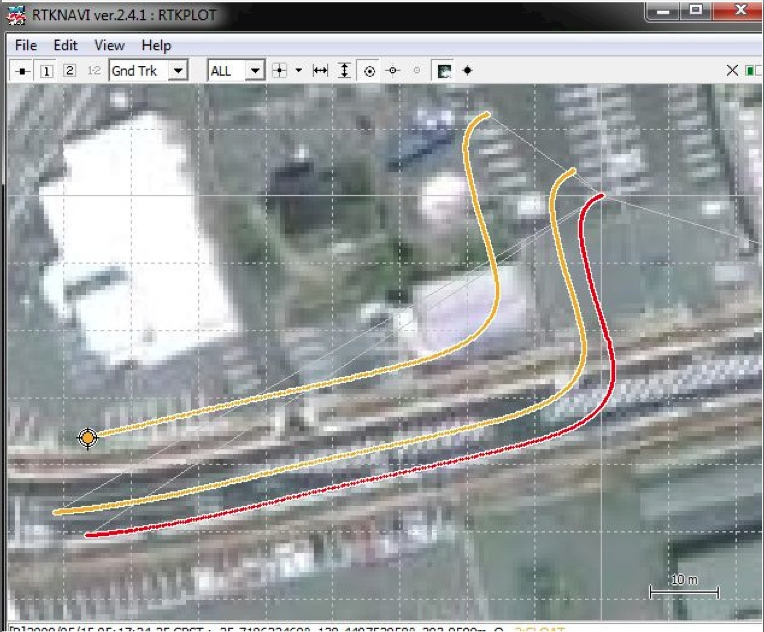
\includegraphics[scale=0.3]{controlledShiftUsingRTCM1005.jpeg}\\
	\caption{Correction Offset}
\end{figure}

When an Ntrip Client requested correction data from the compromised NetRS,
a chain of events happened.  First, the client requested correction data
from the Ntrip Caster about the NetRS mountpoint.  The Ntrip Caster
subsequently queries the Ntrip Server for the latest RTCM3 stream.  The
Ntrip Server then sends the RTCM3 stream it is receiving from the
compromised NetRS mountpoint to the caster, and the caster forwards the
correction data to the client.  The Ntrip Client calculates its position
based on this correction data.  Our attack successfully shifts the client
receiver by an amount directly proportional to the amount of our modification
to the RTCM data.  Figure three shows how a client is affected by the
attack with the red stream indicating the original path without corrections
applied and the yellow paths indicating two different instances of streams
of correction data from the compromised NetRS.

\subsection{Attack Mitigations}

The Ntrip network should be resilient to attack for reliable GPS correction
data.  One technique that could reduce the impact of the aforementioned
attack would be the use of an integrity monitor.  The integrity monitor
would make sure that correction data is within a a specified bound.  Having
an integrity monitor would catch correction data outside the given good
bound from either an attack or a malfunctioning device.  The Coast Guard's
NDGPS makes use of integrity monitors\cite{NDGPS1}.

All authentication traffic should be encrypted.  Allowing passwords to be
transmitted in plaintext or base-64 encoding should be eliminated from the
Ntrip system.  Also, mutual authentication should occur between entities in
the Ntrip network to thwart Man in the Middle attacks.

Future research should include additional research into attack mitigations
as well as their effect on the Ntrip network.

\section{Scope of Impact}

Both the attack created in this research as well as the other attacks mentioned
show the high level of vulnerability in DGPS.  Anyone with knowledge of these
attacks could remotely manipulate DGPS information around the world.
Therefore, any application that relies on DGPS is at risk of receiving
incorrect location information at any time.  This could have far reaching
effects on many people.  The results could range from a loss of time and money
to physical danger and human death.

The attack outlined in this paper was crafted specifically for the Trimble
NetRS reference station, and as such the results are limited to that device.
However, the Trimble NetRS is the most widely deployed Reference Station
that can be found through the master NtripCaster list on rtcm-ntrip.org.
Out of 4995 Reference Stations, 1126 were Trimble NetRS devices, vulnerable
to the attack outlined in this paper.  

Further digging also shows that the sources in the field are indeed vulnerable
in other ways as well.  Out of the 4995 reference stations, 4994 use basic
authentication with nothing more than base-64 encoding to protect username
and passwords.  Only one reference stations uses the stronger digest authentication to provide any protection from snooping passwords.

\section{Future Work}

During the course of this research, a lot of questions came up that we simply didn't have enough time to answer.  In the future, we would like do further research into Virtual Reference Station networks which are networks of reference stations serving to provide even more precise position data over a wider geographical area.  We are interested in whether these networks would "average out" corrupted correction streams or not.

We were also unable to determine whether or not differential corrections are applied to a receivers time calculations or not.  This would certainly be an important area of focus for future research.

We would also like to perform a security assessment of alternative DGPS standards such as the NDGPS, WAAS, and others as well as investigate whether or not any real life attacks against differential GPS have ever occurred and what the objectives were.

\section{Conclusion}

We have discovered a Differential GPS system that is widely used yet highly insecure.  It is important for all users and implementors of differential GPS technologies to make security more of a priority as cyberphysical security is an area of active research and interest.  Ntrip, in particular, is used in many applications requiring DGPS for extremely accurate location measuring.  We showed many instances of users using Ntrip, provided a taxonomy of weaknesses, demonstrated an attack against an Ntrip network running an RTK Engine, and provided the scope of impact of these weaknesses.

The weaknesses seen in Ntrip bring into question the security of differential GPS as a whole.  Many applications require DGPS, and the implications of an attacker with the capability to transmit arbitrary correction data that is accepted as correct by an end user could have dire consequences.  The addition of integrity monitors, mutual authentication, and encryption add additional security to DGPS and thwart many of the existing attacks.  We believe the unveiling of weaknesses in DGPS will spring forth an exciting research area, and shed light onto how to better secure DGPS.

\section{Thanks}

Dr. Georg Weber for providing helpful links and commentary on the adoption of Ntrip in geodetic equipment.
Jeff Jalbrzikowski for providing valuable guidance regarding real life applications of Differential GPS and GPS in the context of Surveying.
Tyler Nyswander for sharing his efforts in gaining root access to the NetRS device.

\section{Appendix A - Tables}

\begin{center}
\begin{tabular}{|c|c|}
  \hline
  Manufacturer & Number of Devices \\
  \hline
  \hline
  AOA & 41\\
  \hline
  Aquarius & 1\\
  \hline
  AshTech & 122\\
  \hline
  BNC & 7\\
  \hline
  BNS & 10\\
  \hline
  EPOS & 41\\
  \hline
  EuroConf & 65\\
  \hline
  EuroNet & 15\\
  \hline
  GNSMART & 1\\
  \hline
  Javad & 178\\
  \hline
  Leica & 1191\\
  \hline
  Magellan & 2\\
  \hline
  Navis & 3\\
  \hline
  Novatel & 3\\
  \hline
  Septentrio & 25\\
  \hline
  Sokkia & 12\\
  \hline
  Topcon & 190\\
  \hline
  Thales & 12\\
  \hline
  Trimble & 2785\\
  \hline
  Unknown & 385\\
  \hline
  Total & 5089\\
  \hline
\end{tabular}\\
Table 1 - Number of Reference Station Devices by Manufacturer
\vspace{10mm}

\begin{tabular}{|c|c|}
  \hline
  Trimble Device & Number of Devices\\
  \hline
  \hline
  TRIMBLE 4000SSI & 2\\
  \hline
  TRIMBLE 4700 & 38\\
  \hline
  TRIMBLE NETR5 & 262\\
  \hline
  TRIMBLE NETR8 & 54\\
  \hline
  TRIMBLE NETR9 & 67\\
  \hline
  TRIMBLE NETRS & 1126\\
  \hline
  TRIMBLE R7 & 8\\
  \hline
  Trimble & 13\\
  \hline
  Trimble 4000 & 3\\
  \hline
  Trimble 5700 & 112\\
  \hline
  Trimble 5700R7 & 2\\
  \hline
  Trimble BD982 & 4\\
  \hline
  Trimble GPSBase & 1\\
  \hline
  Trimble GPSNet & 638\\
  \hline
  Trimble NetR3 & 2\\
  \hline
  Trimble ProXRT & 1\\
  \hline
  Trimble R7 & 6\\
  \hline
  Trimble SPS850 & 1\\
  \hline
  Trimble SPS852 & 1\\
  \hline
  Trimble VRSNet & 444\\
  \hline
\end{tabular}\\
Table 2 - Number and Types of Trimble Reference Stations
\vspace{10 mm}


\begin{tabular}{|c|c|}
  \hline
  Devices w/ Basic Authentication & Devices w/ Digest Authentication\\
  \hline
  \hline
  4994 & 1\\
  \hline
\end{tabular}

Table 3 - Authentication Schemes of Reference Stations
\vspace{10 mm}

\begin{tabular}{|c|c|}
  \hline
  Streams Charging a Fee & Streams Charging No Fee\\
  \hline
  \hline
  867 & 4129\\
  \hline
\end{tabular}
\\

Table 4 - Billing Status of Ntrip Streams

\end{center}

\bibliographystyle{plain}
\bibliography{biblio}
\end{document}


